\section*{Literaturübersicht}
Es wurden bereits Zahlreiche Versuche unternommen das trainiren von HMMs durch Einbinden von Metaheuristiken zu verbessern. Darunter befinden sich Hybridisierungen mit klassischen Metaheuristiken wie Ant Colony Optimization \cite*{LiteratureReviewACO} und Simulated Annealing \cite*{LiteratureReviewSA} aber auch neuere metapher-basierte Metaheuristiken wie modified gravitational search \cite*{LiteratureReviewMGS}, Artificial Bee Colony \cite*{LiteratureReviewABC} und chaos optimization \cite*{LiteratureReviewCO} wurden auf das Problem der HMM Parameter optimierung angewendet. Es existieren sogar Ansätze, in welchen zwei Metaheuristiken mit dem Baum-Welch Algorithmus hybridisiert werden. Der GATSBW Algorithmus \cite*{LiteratureReviewGATSBW} zum Beispiel ist eine Kombination aus genetischen Algorithmus, Tabu-Suche und Baum-Welch Algorithmus. Neben dem erlernen der Parameter wurden Metaheuristiken ebenfalls verwendet um eine passende Struktur (Anzahl der Zustände) zu finden \cite*{LiteratureReviewStructure}.

Die Metaheuristischen Parameterestimationsverfahren lassen sich meinen Beobachtungen nach in drei Kategorien unterteilen.
\begin{itemize}
    \item Rein metaheuristisch: Die Parameter werden nur durch eine Metheuristik erlernt. Es kommt keine lokale Suche zum Einsatz.
    \item Erst Metaheuristik, dann BW: Die Metaheuristik wird verwendet um initiale Parameter für den Baum-Welch Algorithmus zu bestimmen (Relay-Hybrid).
    \item Metaheuristik und BW gleichzeitig: Eine Populationsbasierte Metaheuristik leitet die globale Suche. Lösungen werden mittels Baum-Welch intensiviert (Teamwork-Hybrid) 
\end{itemize}
Aus den existierenden Ansätzen welche Hidden Markov Modelle mittels eines genetischen Algorithmus trainieren wurde für jede dieser drei Kategorien ein Ansatz herausgesucht.


\section{Implementierung}
Die ursprüngliche Idee zur Implementation eines GA-HMM Frameworks war es bereits existierende Python Libraries für HMMs und Genetische Algorithmen zu kombinieren. Da ich jedoch keine Libraries gefunden habe, welche meinen hohen Ansprüchen an Erweiterbarkeit genügten habe ich den Code von Grund auf konstruiert. Meine Erfahrung, des aus dieser Entscheidung resultierenden Schaffensprozesses, lässt sich adäquat durch folgendes Zitat beschreiben.
"The basic idea behind the from scratch-oriented approach is the apparent simplicity of metaheuristic code. Programmers are tempted to develop themselves their codes. Therefore, they are faced with several problems: the development requires time and energy, and it is error prone and difficult to maintain and evolve" \cite*{MetaheuristicsEGT}
Im folgenden werde die Funktionsweise des Frameworks beschreiben und darauf eingehen was bei einer Kombination von Hidden Markov Modellen mit einem genetischen Algorithmus zu beachten ist.

\subsection*{Representation}
Wir erinnern uns, dass bei einem genetischen Algorithmus die Parameter in eine genetische Representation (Chromosom) überführt werden müssen. Die am häufigsten verwendete genetische Representation von HMM Parametern ist es die Matrizen der Parameter zu linearisieren und zu konkatenieren. Auch in dieser Arbeit werden wir solch eine Representation verwenden. Neben den parametern des Hidden Markov Models werden noch zusätzliche Informationen als Gene Kodiert. Darunter sind Fitness und Rang so wie Anzahl der Zustände und Anzahl der Emissionssymbole. Die Anzahl der Zustände und Emissionsymbole werden als Gene kodiert, damit diese bei der Überführung von Chromosom-Representation zu HMM-Representation nicht als Parameter übergeben werden müssen. Die Kodierung der Fitness und des Rangs als Gene folgt einem ähnlichen Rational.
\begin{figure}[h!]
    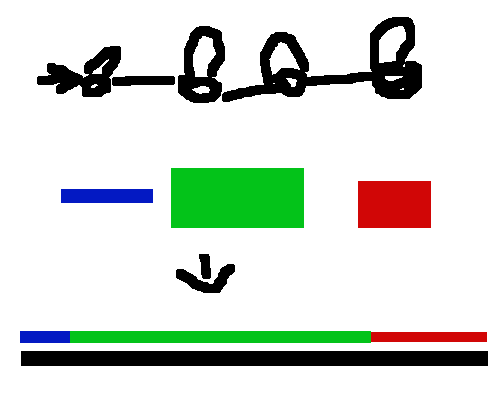
\includegraphics[scale=1.0]{images/Hmm_Chromosom_Representation.png}
    \caption{genetische Representation eines HMM}
    \label{fig:hmm_genetic_representation}
\end{figure}

\subsection*{Die Fitness Funktion}
Unser Ziel ist Parameter $\lambda = \pi, B, A$ zu finden welche die Wahrscheinlichkeit einer Menge an Observationssequenzen maximieren. Die Fitness Funktion eines Chromosoms ist daher die durchschnittliche Log-Wahrscheinlichkeit der Observationssequenzen für den Phänotyp des Chromosoms.
\begin{equation*}
    fitness(\lambda) = \frac{\sum_{\text{alle O}} log[P(O \mid \lambda)] }{\text{anzahl O}} 
\end{equation*}


\subsection*{Genetische Operatoren}
Die Genetischen Operatoren welche implementiert wurden sind

\subsubsection*{Crossover Operatoren}


\subsubsection*{Mutations Operatoren}
Um zu garantieren, dass die Struktur eines Hidden Markov Models nicht verändert wird gibt es verschiedene Kategorien.
- Nur Emissionsmatrix mutieren
- Maske erstellen und nur maskierte Werte Mutieren
- Werte die Nicht verändert werden dürfen nicht in die Chromosom-Representation aufnehmen.

\subsection*{Ablauf des GA-HMM}
Der GA-HMM erweitert den Ablauf eines klassischen genetischen Algorithmus um einige Schritte. Durch den Reproduktionsschritt können Chromosome erzeugt werden, welche unzulässige HMM-Parameter representieren. Zum Beispiel kann durch eine Mutation oder ein Crossover die Reihenstochastizität verletzt werden. Um solche unzulässigen Repräsentationen in den folgenden Schritten zu verhindern folgt nach dem Reproduktionsschritt ein \textbf{Normalisierungs-Schritt}. Solch eine Transformation unzulässiger Lösung in zulässige Lösungen ist bekannt als \textbf{Reparatur Strategie} \cite*{MetaheuristicsEGT}. Des weiteren findet vor der Normalisierung ein optionaler \textbf{Smoothing-Schritt} statt um Overfitting entgegenzuwirken. Der Baum-Welch Algorithmus kann vor dem genetischen Algorithmus, danach und zwischendurch angewendet werden. Dadurch sind Relay-Hybridisierung, Teamwork-Hybridisierung und auch keine Hybridisierung innerhalb eines Frameworks durch Parameter für die einzelnen Baum-Welch Schritte realisierbar.

\begin{figure}[h!]
    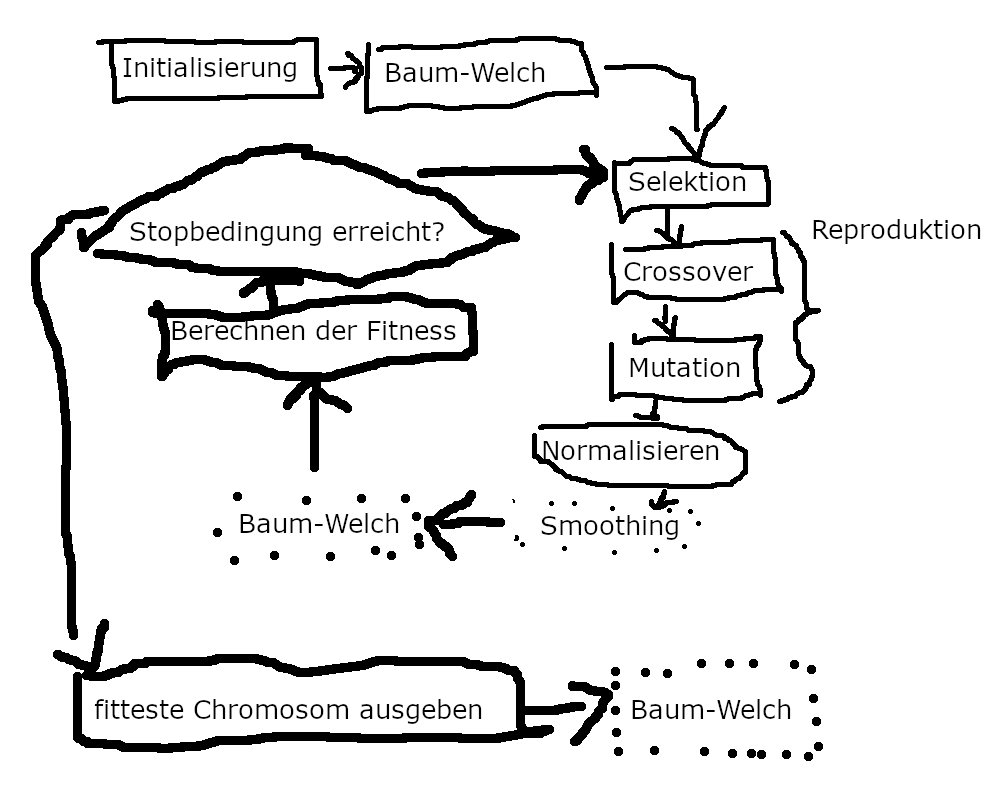
\includegraphics[scale=1.0]{images/GA-HMM_Flowchart.png}
    \caption{Ablauf des GA-HMM}
    \label{fig:gahmm_flowchart}
\end{figure}

\subsection*{Trainingsdaten}
Zum Evaluieren der verschiedenen Trainingsverfahren wurden zwei Datensätze erstellt. Ein Datensatz wurde aus sprachlichen Äußerungen der Zahlen 0 bis 9 erstellt. Dazu wurden die Audiodateien zunächst in eine Vektorrepresentation überführt. Sogenannte \textbf{Mel Frequency Cepestral Coefficients (MFCCs)}. Dabei handelt es sich um eine Darstellung des Frequenzspektrums welche dem menschlichen Hören nachempfunden ist. Diese MFCC-Vektoren wurden dann mit einem k-means Algorithmus quantisiert so dass man Observationssequenzen mit diskreten Symbolen erhält. Die Audiodateien wurden aus dem Free Spoken Digit Dataset (FSDD) entnommen. Ein zweiter Datensatz wurde aus Schwarz-Weiß Bildern von Gesichertern aus der ORL-Faces Datenbank generiert. Dazu wurden die Bilder zunächst linearisiert und anschließend wurden die Auflösung der Grau-Werte verringert um nicht allzuviele Emissionsymbole zu erhalten.

\subsection*{Implementation des Baum-Welch}
% Korrektheit der Implementation wurde verifiziert durch stamp
% Mehrere Auxiliary methoden zum trainieren mehrerer hmms gleichzeitig
Der Baum-Welch Algorithmus wurde ebenfalls in python implementiert. Mittels des Numba JIT Compilers wird dieser Python-Code während der Laufzeit zu hochperformanten C-Code kompiliert. Um Kompilationszeit bei einem initialen Funktionsaufruf zu umgehen wird der kompilierte C-Code gecached. Die Korrektheit der Implementation wurde verifiziert indem ein HMM mit der gleiche Observationssequenz und gleichen initialen Parametern wie in Stamp [HIER STAMP REF EINFÜGEN] trainiert wurde. Die trainierten Parameter meiner Implementation weichen von den trainierten Parametern in Stamp um weniger als 0.0001 ab, was nach 100 Iterationen wohl im Bereich der durch Systemunterschiede erklärbaren Diskrepanz liegt.

\subsection*{Testing}
Um die Korrektheit der Implementation des GA-HMM zu verifizieren wurde ein Domänenspezifisches Test-Framework entwickelt. Die domänenspezifischen Methoden ermöglichen unter anderem Assert-Statements über Validität, Equivalenz- und Ähnlichkeit der HMM und Chromosom Datentypen zu machen. Dadurch ist eine übersichtliche Validierung des Codes möglich.